\documentclass[11pt,a4paper]{article}
\usepackage[T1]{fontenc}
\usepackage{lmodern}
\usepackage[margin=2.4cm]{geometry}
\usepackage{booktabs}
\usepackage{longtable}
\usepackage{url}
\usepackage{graphicx}
\usepackage{tikz}
\usetikzlibrary{arrows.meta,positioning,calc}
\graphicspath{{../../.local/review/v4.0/}}
\newcommand{\shot}[3]{%
\begin{figure}[htbp]\centering
\includegraphics[width=#2\linewidth]{#1}
\caption{#3}
\end{figure}}
\setlength{\parindent}{0pt}
\setlength{\parskip}{0.55em}
\renewcommand{\arraystretch}{1.2}

\title{Hiep Trong Space v4.0\\[0.3em]\large Writing Room, Current Focus and Learning Room}
\author{Implementation report}
\date{18 November 2026}

\begin{document}
\maketitle

\section{Summary}
Version 4.0 renames two pages and rebuilds three features, using every recommended answer from the v4.0 proposal. The checks at the end of the work were clean: lint, type check and 495 tests passed, and the production build succeeded. Nothing is committed. The working tree also still holds earlier uncommitted changes.

\section{Renames and routes}
\begin{tabular}{@{}lll@{}}
\toprule
Old name & New name & Route \\
\midrule
Blogs Hub & Writing Room & \texttt{/writing} (\texttt{/blogs} redirects) \\
In Progress Projects & Current Focus & \texttt{/focus} (\texttt{/projects} redirects) \\
\bottomrule
\end{tabular}

Feature ids, theme names and API paths are unchanged. The redirects are permanent and live in \texttt{next.config.ts}.

\section{Writing Room}
\subsection{Shelf and rooms}
The main page shows three 3D books on a cabin shelf: a kraft notebook (Draft Room), a cloth hardcover (My Perspective) and a leather diary (Private Room). Clicking a book swings the cover open for about one second, then navigates to the room. Reduced motion skips the wait. The unused lantern artwork glows on days something was written.

\begin{itemize}
\item \textbf{Draft Room:} index cards, Seed/Sprout/Ready ripeness, a ``From the drawer'' note that resurfaces an old draft, and clippings.
\item \textbf{My Perspective:} contents page, a question per essay, dated margin notes, revisit dates, and a Read mode.
\item \textbf{Private Room:} password gate, diary, reflection and recap entries with prompts, a ``today's sky'' mood, ``on this day'', and weekly or monthly recaps pre-filled from tasks and study time.
\end{itemize}

\shot{shelf.jpg}{0.9}{The Writing Room shelf: three bound books, a tag under each, and the lantern (unlit because nothing was written that day).}

\shot{draft.jpg}{0.9}{A migrated clipping open in Draft Room: page icon, ripeness and tags, formatting toolbar, outline and word count in the right rail.}

\shot{contents.jpg}{0.9}{My Perspective contents page, listing each essay by the question it answers.}

\subsection{Editor}
Every page uses a TipTap-based Notion-style editor: slash menu, \texttt{@} page links, markdown shortcuts, headings, lists, to-do, toggle, quote, callout, divider, image by URL, selection toolbar, sub-pages, outline, backlinks, sidebar tree, favorites, a 30-day trash and autosave. Drag handles, databases and table views are not built.

\shot{slash.jpg}{0.8}{The slash menu opened at the caret, listing block types.}

\subsection{Private Room security}
Entries are encrypted with AES-256-GCM. A random master key is wrapped twice: once by a key derived with scrypt from the password, and once by a key derived from a one-time recovery code. The password is never stored. Sessions are held in server memory, use an \texttt{httpOnly} \texttt{SameSite=Strict} cookie, and expire after 10 idle minutes. Five failed attempts pause unlocking for 60 seconds. Everything is stored under the Git-ignored \texttt{data/} folder, and a test fails if any private file is tracked. Losing both the password and the recovery code makes entries unrecoverable.

\begin{figure}[htbp]\centering
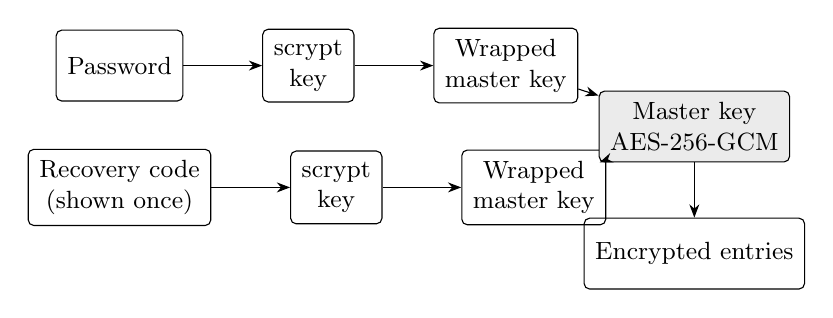
\begin{tikzpicture}[font=\small,
  box/.style={draw,rounded corners=2pt,minimum height=0.9cm,align=center,inner sep=4pt},
  >=Stealth]
\node[box] (pw) {Password};
\node[box,below=0.6cm of pw] (rc) {Recovery code\\(shown once)};
\node[box,right=1cm of pw] (k1) {scrypt\\key};
\node[box,right=1cm of rc] (k2) {scrypt\\key};
\node[box,right=1cm of k1] (w1) {Wrapped\\master key};
\node[box,right=1cm of k2] (w2) {Wrapped\\master key};
\node[box,fill=black!8,right=1cm of $(w1)!0.5!(w2)$] (mk) {Master key\\AES-256-GCM};
\draw[->] (pw)--(k1); \draw[->] (rc)--(k2);
\draw[->] (k1)--(w1); \draw[->] (k2)--(w2);
\draw[->] (w1)--(mk); \draw[->] (w2)--(mk);
\node[box,below=0.7cm of mk] (en) {Encrypted entries};
\draw[->] (mk)--(en);
\end{tikzpicture}
\caption{Either secret unwraps the same random master key, which encrypts every entry. The wrapped keys and the entries live under the Git-ignored \texttt{data/} folder.}
\end{figure}

\shot{private.jpg}{0.7}{The Private Room on first visit: the password is set before anything can be written.}

\subsection{Migration}
On first load, old Blogs Hub articles are copied once: drafts to Draft Room, published articles to My Perspective, and saved-from-others as Draft Room clippings. A marker file prevents a second import.

\section{Current Focus}
Records gain a one-line reason, checkpoints that drive progress, parking details, a weekly note and a finish date. The card shows a pace marker (Ahead, On pace, Behind), linked tasks done, focus time from Learning Room, last-moved, an eight-week pulse chart and a Quiet state after 14 days. Statuses become In focus, On deck, Parked and Finished, and old values map across on read (Figure~\ref{fig:status}).

\begin{figure}[htbp]\centering
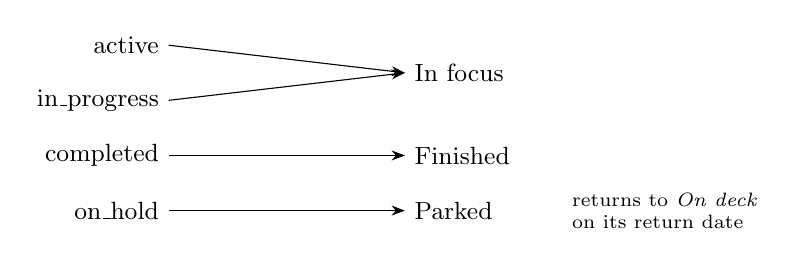
\begin{tikzpicture}[font=\small,>=Stealth]
\node[anchor=east] (a1) at (0,0) {active};
\node[anchor=east] (a2) at (0,-0.7) {in\_progress};
\node[anchor=east] (a3) at (0,-1.4) {completed};
\node[anchor=east] (a4) at (0,-2.1) {on\_hold};
\node[anchor=west] (b1) at (3,-0.35) {In focus};
\node[anchor=west] (b3) at (3,-1.4) {Finished};
\node[anchor=west] (b4) at (3,-2.1) {Parked};
\draw[->] (a1.east)--(b1.west);
\draw[->] (a2.east)--(b1.west);
\draw[->] (a3.east)--(b3.west);
\draw[->] (a4.east)--(b4.west);
\node[anchor=west,font=\scriptsize,align=left] at (5,-2.1) {returns to \textit{On deck}\\on its return date};
\end{tikzpicture}
\caption{Legacy status words and their v4.0 equivalents. \textit{On deck} is new.}\label{fig:status}
\end{figure} More than three active focuses shows a warning, never a block. Locally saved drafts from before v4.0 still resume without wiping linked tasks.

\shot{focus.jpg}{0.9}{Current Focus with no records yet: status filters and the training-dummy empty state.}

\section{Learning Room}
The subject picker is removed. A session starts from a task or as a free session, takes a name, and splits the total time into focus blocks and breaks that can be adjusted one at a time. The browser tab title shows the countdown and flashes an alert with a red icon dot when a phase ends in a hidden tab. A refresh resumes a running session. Also added: parked thoughts (press P), break cards, and an option to mark the task done when finishing. Time is now broken down by Current Focus.

\begin{figure}[htbp]\centering
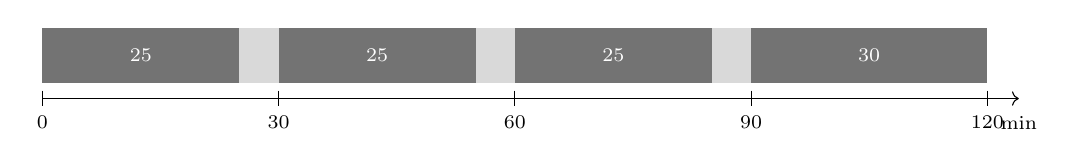
\begin{tikzpicture}[x=0.1cm,font=\scriptsize]
\fill[black!55] (0,0) rectangle (25,0.7);   \node[white] at (12.5,0.35) {25};
\fill[black!15] (25,0) rectangle (30,0.7);
\fill[black!55] (30,0) rectangle (55,0.7);  \node[white] at (42.5,0.35) {25};
\fill[black!15] (55,0) rectangle (60,0.7);
\fill[black!55] (60,0) rectangle (85,0.7);  \node[white] at (72.5,0.35) {25};
\fill[black!15] (85,0) rectangle (90,0.7);
\fill[black!55] (90,0) rectangle (120,0.7); \node[white] at (105,0.35) {30};
\draw[->] (0,-0.2)--(124,-0.2);
\foreach \t in {0,30,60,90,120} \draw (\t,-0.1)--(\t,-0.3) node[below] {\t};
\node[below] at (124,-0.3) {min};
\end{tikzpicture}
\caption{Default plan for a 120-minute total: dark blocks are focus, light blocks are 5-minute breaks. A remainder too small for a break is folded into the last block (30 minutes).}
\end{figure}

\shot{learning.jpg}{0.9}{Learning Room setup: task picker built from open tasks, session name, total-time slider and block steppers.}

\section{Shared changes}
\begin{itemize}
\item Newsreader font for reading and writing surfaces, and a soft emerald text selection app-wide.
\item A shared tab-title helper (\texttt{src/client/tab-title.ts}).
\item New design tokens for book bindings, paper and shelf wood.
\item Engineering document updated with a v4.0 section.
\end{itemize}

\section{Deviations and gaps}
\begin{longtable}{@{}p{0.3\linewidth}p{0.66\linewidth}@{}}
\toprule
Item & Outcome \\
\midrule
\endhead
Search shortcut & \texttt{Ctrl+K} already opens the Universe menu, so search uses \texttt{/}. \\
Quick note shortcut & Browsers reserve \texttt{Ctrl+Shift+N}, so quick note uses \texttt{Alt+N}. \\
Block drag handles & Not built. \\
Phase-change sound & Not built (it was off by default). \\
New line-art assets & Not drawn. Existing unused art was put to use instead. \\
\bottomrule
\end{longtable}

\section{Verification}
\textbf{Automated:} lint, type check and 495 tests pass, including new tests for study plans and sessions, focus pace and quiet logic, the writing service and migration, and the vault (encryption on disk, lockout, idle lock, recovery, and a Git guard). \texttt{npm run build} succeeds.

\textbf{In a browser:} the shelf, Draft Room, My Perspective, slash menu, Learning Room setup, Current Focus page and the redirect.

\textbf{Not tried in a browser:} Private Room setup end to end (the real vault was left untouched), tab-title alerts in a hidden tab, \texttt{Alt+N}, and the selection toolbar. Three unrelated tests timed out once under full-suite load and passed alone and on the final run.

\section{Data touched}
The first visit to \texttt{/writing} creates \texttt{data/writing-pages.json} and \texttt{data/writing-meta.json} from existing blog articles. During testing these were deleted and re-created once so headings imported correctly. The old \texttt{/api/blogs} routes remain as the import source.

\end{document}
